\section{Introduction}
%  task description

%Visual relationship detection (VRD) \cite{Lu16} is an important task in computer vision domain. Because scene graph is the most common used structure to describe the visual relationship in the most of recent works, , it is often referred as Scene graph generation (SGG) \cite{scene-graph}. 
% Scene graph generation aims to understand the semantic content of an image via a scene graph, where nodes indicate  visual objects and edges indicate pairwise object relationships. An intuitive example of scene graph generation is shown in Figure~\ref{fig:sgg_sample}. Scene graph generation is very helpful for computer to bridge the gap between the low-level visual perceiving data and the high-level semantic description. Therefore, a reliable scene graph can provide powerful support for downstream tasks such as image captioning~\cite{Zhong2020Comprehensive}, image retrieval~\cite{scene-graph}, and visual question answering~\cite{VCTree_tang}. 

Scene graph generation aims to understand the semantic content of an image via a scene graph, where nodes indicate visual objects and edges indicate pairwise object relationships. An intuitive example of scene graph generation is shown in Figure~\ref{fig:sgg_sample}. Scene graph generation is beneficial to bridge the gap between the low-level visual perceiving data and the high-level semantic description. Therefore, a reliable scene graph can provide powerful support for downstream tasks, such as image captioning~\cite{Zhong2020Comprehensive}, image retrieval~\cite{scene-graph}, and visual question answering~\cite{VCTree_tang}. 

\begin{figure}[!ht]
	\centering
	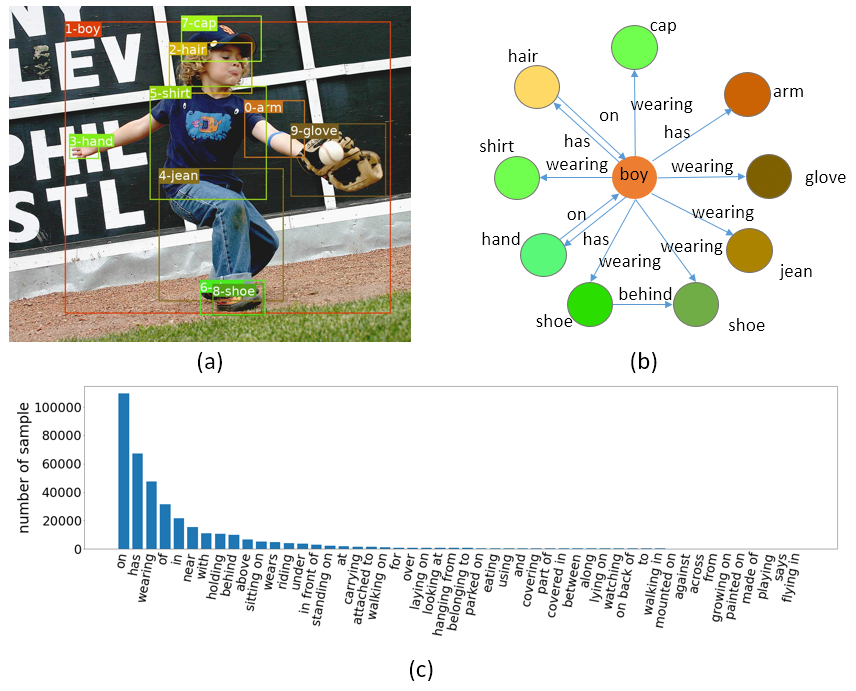
\includegraphics[width=\linewidth]{figure/sgg_sample} %
	\caption{(a) an input image with detected objects. (b) a generated scene graph, which is a graphical representation of the input image with objects and pairwise relationships. (c) the long-tail distribution of object relationships in the Visual Genome (VG) dataset~\cite{krishna2016visual}.}
	\label{fig:sgg_sample}
\end{figure}

%Scene graph generation task usually suffers from the long-tail problem of relationships in training data \cite{Tang2020_unbiased,chen2019knowledge}. 
%For example, as shown in Figure~\ref{fig:sgg_sample}(c), the widely used scene graph generation dataset, i.e., Visual Genome ~\cite{krishna2016visual}, is dominated by a few relationships with coarse-grained descriptions (head categories), while there are no sufficient annotations available for many other less frequent relationships (tail categories). This severe imbalanced distribution makes it difficult for an unbiased scene graph generation. Therefore, it is still a great challenge to enable the model to recognize those less frequent relationships with only a few training samples in real-world scenarios.

Scene graph generation usually suffers from the long-tail problem of relationships in training data \cite{Tang2020_unbiased,chen2019knowledge,zhan2019exploring}. 
For example, as shown in Figure~\ref{fig:sgg_sample}(c), the widely used scene graph generation dataset, Visual Genome ~\cite{krishna2016visual}, is dominated by a few relationships with coarse-grained descriptions (head categories), whereas there are no sufficient annotations available for other less frequent relationships (tail categories). This severe imbalanced distribution makes it difficult for an unbiased scene graph generation, considering there are only a few training samples in real-world scenarios for recognizing less frequent relationships.


% solution.
% \par 
%To address the above-mentioned issues, many class re-balancing strategies have been introduced for unbiased scene graph generation~\cite{Tang2020_unbiased,li2021bipartite}. However, existing methods struggles to achieve a satisfactory trade-off between head and tail categories.
To address the above-mentioned issues, many class re-balancing strategies have been introduced for unbiased scene graph generation~\cite{Tang2020_unbiased,li2021bipartite}. However, existing methods still struggle to achieve satisfactory performance on tail categories, and more sophisticated solutions are desirable. 
%%%%% v1 introduction for trade-off bias %%%%%%%%%
% To explore a way for proper head-tail trade-off, inspired by \cite{Zellers_2018_CVPR}, we further analyze the impact of the external bias item on the model training. 
% And we find out that the bias item can enforce the model to focus on those samples with smaller bias values during the training phase.
% Moreover, in the evaluation period, it encourages the model to output a different distribution from the bias by adjusting the classification boundary. 
% Therefore, the bias can resist the effect of imbalance of training set if we make the distribution of the bias consistent with the data distribution of the training set. 
% We name the external bias as resistance bias (RTB). And we propose several instances of resistance bias that describe the relationship distribution in different manners. By applying our resistance learning scheme, we achieve a better trade-off between head and tail categories than previous work and obtain a balanced model for the unbiased scene graph generation. 
%%%%%%%%%%%%%%%%%%%%%%%%%%%%%%%%%%%%%%%%%%%%%%%%%%
Inspired that humans increase muscle strength by making their muscles work against a force, we propose resistance training using prior bias (RTPB) to improve the detection of less-frequently relationships and address the long-tail problem in SGG.
%, RTPB can adjust the model's feasibility to. 
Specifically, RTPB assigns a class-specific resistance to the model during training, where the resistance on each relationship is determined by a prior bias, named resistance bias. The resistance bias is first initialized by the prior statistic about the relationships in the training set. The motivation of a resistance bias is to enforce the model to strengthen the ability on less frequent relationships, since they are always corresponding to heavier resistance. In this way, RTPB enables the model to resist the influence of the imbalanced training dataset.
% By assign those tail categories in the training set heavier resistance, we can improve the model's feasibility of those less frequently seen relationships.
% experiment for RTPB
Furthermore, to better explore global features for recognizing the relationships, we design a contextual encoding backbone network, named dual Transformer (DTrans for short). Specifically, the DTrans uses two stacks of the Transformer to encode the global information for objects and relationships sequentially. 
% Therefore, DTrans serves as a simple yet effective baseline in our experiments.
To evaluate the effectiveness of the proposed RTPB, we introduce it into recent state-of-the-art methods and our DTrans. Specifically, RTPB can bring an improvement of over 10\% in terms of the mean recall criterion compared with other methods. By integrating with the DTrans baseline, RTPB achieves a new state-of-the-art performance for the unbiased scene graph generation.
% TODO: the connection between RTPB and DT
% \par The RTPB focuses on dealing with the imbalance of training set distribution,
% but the performance still relies on the feature map of the relationship. 
% and a method to analyze the information inside the image is still necessary.
%  The Dual Transformer trained with RTPB achieves state-of-the-art performance.
%To address this problem, we propose the resistance bias module to adjust the training phase of the relationship classifier.

The main contributions of this paper are summarized as follows:
1) We propose a novel resistance training strategy using prior bias (RTPB) to improve the model generalizability on  the rare relationships in the training dataset;
2) We define a general form of resistance bias and devise different types of specific bias by using different ways to model object relationship;
3)   We introduce a contextual encoding structure based on the transformer to form a simple yet effective baseline for scene graph generation.
Extensive experiments on a very popular benchmark demonstrate significant improvements of our RTPB and DTrans compared with many competitive counterparts for unbiased SGG.
